\documentclass[twoside]{book}

% Packages required by doxygen
\usepackage{calc}
\usepackage{doxygen}
\usepackage{graphicx}
\usepackage[utf8]{inputenc}
\usepackage{makeidx}
\usepackage{multicol}
\usepackage{multirow}
\usepackage{fixltx2e}
\PassOptionsToPackage{warn}{textcomp}
\usepackage{textcomp}
\usepackage[nointegrals]{wasysym}
\usepackage[table]{xcolor}

% Font selection
\usepackage[T1]{fontenc}
\usepackage{mathptmx}
\usepackage[scaled=.90]{helvet}
\usepackage{courier}
\usepackage{amssymb}
\usepackage{sectsty}
\renewcommand{\familydefault}{\sfdefault}
\allsectionsfont{%
  \fontseries{bc}\selectfont%
  \color{darkgray}%
}
\renewcommand{\DoxyLabelFont}{%
  \fontseries{bc}\selectfont%
  \color{darkgray}%
}
\newcommand{\+}{\discretionary{\mbox{\scriptsize$\hookleftarrow$}}{}{}}

% Page & text layout
\usepackage{geometry}
\geometry{%
  a4paper,%
  top=2.5cm,%
  bottom=2.5cm,%
  left=2.5cm,%
  right=2.5cm%
}
\tolerance=750
\hfuzz=15pt
\hbadness=750
\setlength{\emergencystretch}{15pt}
\setlength{\parindent}{0cm}
\setlength{\parskip}{0.2cm}
\makeatletter
\renewcommand{\paragraph}{%
  \@startsection{paragraph}{4}{0ex}{-1.0ex}{1.0ex}{%
    \normalfont\normalsize\bfseries\SS@parafont%
  }%
}
\renewcommand{\subparagraph}{%
  \@startsection{subparagraph}{5}{0ex}{-1.0ex}{1.0ex}{%
    \normalfont\normalsize\bfseries\SS@subparafont%
  }%
}
\makeatother

% Headers & footers
\usepackage{fancyhdr}
\pagestyle{fancyplain}
\fancyhead[LE]{\fancyplain{}{\bfseries\thepage}}
\fancyhead[CE]{\fancyplain{}{}}
\fancyhead[RE]{\fancyplain{}{\bfseries\leftmark}}
\fancyhead[LO]{\fancyplain{}{\bfseries\rightmark}}
\fancyhead[CO]{\fancyplain{}{}}
\fancyhead[RO]{\fancyplain{}{\bfseries\thepage}}
\fancyfoot[LE]{\fancyplain{}{}}
\fancyfoot[CE]{\fancyplain{}{}}
\fancyfoot[RE]{\fancyplain{}{\bfseries\scriptsize Generated on Mon Oct 27 2014 22\+:32\+:42 for Qt\+Mock\+Web\+Server by Doxygen }}
\fancyfoot[LO]{\fancyplain{}{\bfseries\scriptsize Generated on Mon Oct 27 2014 22\+:32\+:42 for Qt\+Mock\+Web\+Server by Doxygen }}
\fancyfoot[CO]{\fancyplain{}{}}
\fancyfoot[RO]{\fancyplain{}{}}
\renewcommand{\footrulewidth}{0.4pt}
\renewcommand{\chaptermark}[1]{%
  \markboth{#1}{}%
}
\renewcommand{\sectionmark}[1]{%
  \markright{\thesection\ #1}%
}

% Indices & bibliography
\usepackage{natbib}
\usepackage[titles]{tocloft}
\setcounter{tocdepth}{3}
\setcounter{secnumdepth}{5}
\makeindex

% Hyperlinks (required, but should be loaded last)
\usepackage{ifpdf}
\ifpdf
  \usepackage[pdftex,pagebackref=true]{hyperref}
\else
  \usepackage[ps2pdf,pagebackref=true]{hyperref}
\fi
\hypersetup{%
  colorlinks=true,%
  linkcolor=blue,%
  citecolor=blue,%
  unicode%
}

% Custom commands
\newcommand{\clearemptydoublepage}{%
  \newpage{\pagestyle{empty}\cleardoublepage}%
}


%===== C O N T E N T S =====

\begin{document}

% Titlepage & ToC
\hypersetup{pageanchor=false,
             bookmarks=true,
             bookmarksnumbered=true,
             pdfencoding=unicode
            }
\pagenumbering{roman}
\begin{titlepage}
\vspace*{7cm}
\begin{center}%
{\Large Qt\+Mock\+Web\+Server \\[1ex]\large 1.\+0 }\\
\vspace*{1cm}
{\large Generated by Doxygen 1.8.7}\\
\vspace*{0.5cm}
{\small Mon Oct 27 2014 22:32:42}\\
\end{center}
\end{titlepage}
\clearemptydoublepage
\tableofcontents
\clearemptydoublepage
\pagenumbering{arabic}
\hypersetup{pageanchor=true}

%--- Begin generated contents ---
\chapter{Main Page}
\label{index}\hypertarget{index}{}A mock web server implemented using Qt for testing H\+T\+T\+P clients. This project is inspired by the mock web server in project \href{https://github.com/square/okhttp/tree/master/mockwebserver}{\tt okhttp}, with small changes to A\+P\+I names to make it a bit more Qt style. Thanks to their great work!

\subsubsection*{Example}

\begin{DoxyVerb}```cpp
// Create a QtMockWebServer.
QtMockWebServer server;

// Schedule some responses.
server.enqueue(MockResponse().setBody("hello, world!"));
server.enqueue(MockResponse().setBody("sup, bra?"));
server.enqueue(MockResponse().setBody("yo dog"));

// Start the server.
server.play();

// Ask the server for its URL. You'll need this to make HTTP requests.
QUrl baseUrl = server.getUrl("/v1/chat/");

// Exercise your application code, which should make those HTTP requests.
// Responses are returned in the same order that they are enqueued.
Chat chat = new Chat(baseUrl);

chat.loadMore();
assertEquals("hello, world!", chat.messages());

chat.loadMore();
chat.loadMore();
QCOMPARE(chat.messages(), QString("hello, world!\nsup, bra?\nyo dog"));

// Optional: confirm that your app made the HTTP requests you were expecting.
RecordedRequest request1 = server.takeRequest();
QCOMPARE(request1.path(), QString("/v1/chat/messages/"));
QVERIFY2(!request1.header("Authorization").isEmpty(), "Authorization header is empty.");

RecordedRequest request2 = server.takeRequest();
QCOMPARE(request2.path(), QString("/v1/chat/messages/2"));

RecordedRequest request3 = server.takeRequest();
QCOMPARE(request3.path(), QString("/v1/chat/messages/3"));

// Shut down the server. Instances cannot be reused.
server.shutdown();
```
\end{DoxyVerb}


\subsubsection*{T\+O\+D\+O}


\begin{DoxyItemize}
\item H\+T\+T\+P\+S support.
\item Throttle control.
\end{DoxyItemize}

\subsubsection*{License}

\begin{DoxyVerb}Licensed under the Apache License, Version 2.0 (the "License");
you may not use this file except in compliance with the License.
You may obtain a copy of the License at

   http://www.apache.org/licenses/LICENSE-2.0

Unless required by applicable law or agreed to in writing, software
distributed under the License is distributed on an "AS IS" BASIS,
WITHOUT WARRANTIES OR CONDITIONS OF ANY KIND, either express or implied.
See the License for the specific language governing permissions and
limitations under the License.\end{DoxyVerb}
 
\chapter{Todo List}
\label{todo}
\hypertarget{todo}{}

\begin{DoxyRefList}
\item[\label{todo__todo000001}%
\hypertarget{todo__todo000001}{}%
Member \hyperlink{class_qt_mock_web_server_a9b3f8f6054887c147b2c3fb36fbce271}{Qt\+Mock\+Web\+Server\+:\+:set\+Body\+Limit} (int max\+Body\+Length)]Not fully implemented.  
\item[\label{todo__todo000003}%
\hypertarget{todo__todo000003}{}%
Member \hyperlink{class_queue_dispatcher_ab7a07e38d21032f2657896c647cb6f2f}{Queue\+Dispatcher\+:\+:set\+Fail\+Fast} (\hyperlink{class_mock_response}{Mock\+Response} $\ast$fail\+Fast\+Response)]It will be useful after queue is implemented blockable.  
\item[\label{todo__todo000002}%
\hypertarget{todo__todo000002}{}%
Member \hyperlink{class_queue_dispatcher_a2f09193b180fb46fe7b0822022b52222}{Queue\+Dispatcher\+:\+:set\+Fail\+Fast} (bool fail\+Fast)]It will be useful after queue is implemented blockable. 
\end{DoxyRefList}
\chapter{Hierarchical Index}
\section{Class Hierarchy}
This inheritance list is sorted roughly, but not completely, alphabetically\+:\begin{DoxyCompactList}
\item \contentsline{section}{Dispatcher}{\pageref{class_dispatcher}}{}
\begin{DoxyCompactList}
\item \contentsline{section}{Queue\+Dispatcher}{\pageref{class_queue_dispatcher}}{}
\end{DoxyCompactList}
\item \contentsline{section}{Mock\+Response}{\pageref{class_mock_response}}{}
\item Q\+Object\begin{DoxyCompactList}
\item \contentsline{section}{Qt\+Mock\+Web\+Server}{\pageref{class_qt_mock_web_server}}{}
\end{DoxyCompactList}
\item \contentsline{section}{Recorded\+Request}{\pageref{class_recorded_request}}{}
\end{DoxyCompactList}

\chapter{Class Index}
\section{Class List}
Here are the classes, structs, unions and interfaces with brief descriptions\+:\begin{DoxyCompactList}
\item\contentsline{section}{\hyperlink{class_dispatcher}{Dispatcher} \\*Abstract parent of dispatchers }{\pageref{class_dispatcher}}{}
\item\contentsline{section}{\hyperlink{class_mock_response}{Mock\+Response} \\*The mock response to be sent to client }{\pageref{class_mock_response}}{}
\item\contentsline{section}{\hyperlink{class_qt_mock_web_server}{Qt\+Mock\+Web\+Server} \\*A mock web server serving requests using pre-\/queued mock responses by default }{\pageref{class_qt_mock_web_server}}{}
\item\contentsline{section}{\hyperlink{class_queue_dispatcher}{Queue\+Dispatcher} \\*A dispatcher using queue policy }{\pageref{class_queue_dispatcher}}{}
\item\contentsline{section}{\hyperlink{class_recorded_request}{Recorded\+Request} \\*The recorded request to be validated }{\pageref{class_recorded_request}}{}
\end{DoxyCompactList}

\chapter{Class Documentation}
\hypertarget{class_dispatcher}{\section{Dispatcher Class Reference}
\label{class_dispatcher}\index{Dispatcher@{Dispatcher}}
}


Abstract parent of dispatchers.  




{\ttfamily \#include $<$Dispatcher.\+h$>$}

Inheritance diagram for Dispatcher\+:\begin{figure}[H]
\begin{center}
\leavevmode
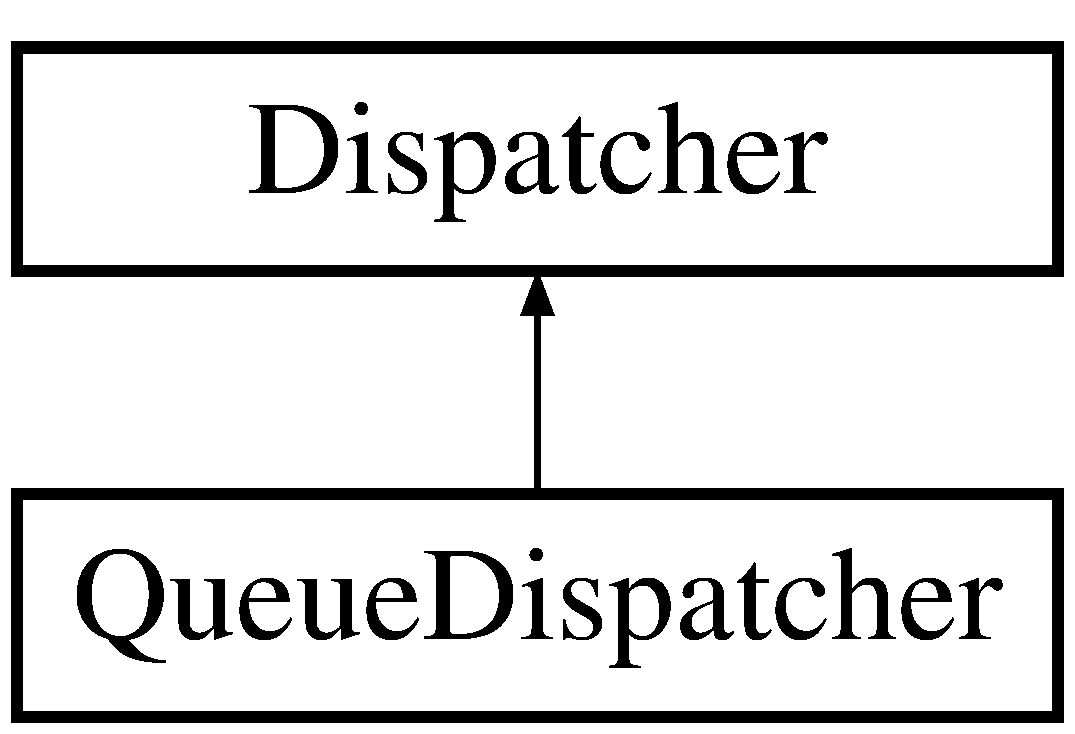
\includegraphics[height=2.000000cm]{class_dispatcher}
\end{center}
\end{figure}
\subsection*{Public Member Functions}
\begin{DoxyCompactItemize}
\item 
virtual \hyperlink{class_mock_response}{Mock\+Response} \hyperlink{class_dispatcher_acbbf8d0ca649be337d805dcbaf4ba81b}{dispatch} (const \hyperlink{class_recorded_request}{Recorded\+Request} \&request)=0
\begin{DoxyCompactList}\small\item\em Dispatch a request. \end{DoxyCompactList}\item 
virtual \hyperlink{class_mock_response}{Mock\+Response} \hyperlink{class_dispatcher_af4768d8abe65389a5cdbb48499c32a0f}{peek} ()
\begin{DoxyCompactList}\small\item\em An early guess of the next response, used for policy on how an incoming requests should be received. \end{DoxyCompactList}\end{DoxyCompactItemize}


\subsection{Detailed Description}
Abstract parent of dispatchers. 

A dispatcher decides what \hyperlink{class_mock_response}{Mock\+Response} should be dispatched giving a \hyperlink{class_recorded_request}{Recorded\+Request}. 

\subsection{Member Function Documentation}
\hypertarget{class_dispatcher_acbbf8d0ca649be337d805dcbaf4ba81b}{\index{Dispatcher@{Dispatcher}!dispatch@{dispatch}}
\index{dispatch@{dispatch}!Dispatcher@{Dispatcher}}
\subsubsection[{dispatch}]{\setlength{\rightskip}{0pt plus 5cm}virtual {\bf Mock\+Response} Dispatcher\+::dispatch (
\begin{DoxyParamCaption}
\item[{const {\bf Recorded\+Request} \&}]{request}
\end{DoxyParamCaption}
)\hspace{0.3cm}{\ttfamily [pure virtual]}}}\label{class_dispatcher_acbbf8d0ca649be337d805dcbaf4ba81b}


Dispatch a request. 


\begin{DoxyParams}{Parameters}
{\em request} & The incoming request. \\
\hline
\end{DoxyParams}
\begin{DoxyReturn}{Returns}
The \hyperlink{class_mock_response}{Mock\+Response} to be sent to client. 
\end{DoxyReturn}


Implemented in \hyperlink{class_queue_dispatcher_ae5fe9ec67b24b75ece3f28d908e2764e}{Queue\+Dispatcher}.

\hypertarget{class_dispatcher_af4768d8abe65389a5cdbb48499c32a0f}{\index{Dispatcher@{Dispatcher}!peek@{peek}}
\index{peek@{peek}!Dispatcher@{Dispatcher}}
\subsubsection[{peek}]{\setlength{\rightskip}{0pt plus 5cm}{\bf Mock\+Response} Dispatcher\+::peek (
\begin{DoxyParamCaption}
{}
\end{DoxyParamCaption}
)\hspace{0.3cm}{\ttfamily [virtual]}}}\label{class_dispatcher_af4768d8abe65389a5cdbb48499c32a0f}


An early guess of the next response, used for policy on how an incoming requests should be received. 

\begin{DoxyReturn}{Returns}
An early guess of the next response. 
\end{DoxyReturn}


Reimplemented in \hyperlink{class_queue_dispatcher_acea23f016b5fd62ec7cc94ee1db1816e}{Queue\+Dispatcher}.



The documentation for this class was generated from the following files\+:\begin{DoxyCompactItemize}
\item 
src/Dispatcher.\+h\item 
src/Dispatcher.\+cpp\end{DoxyCompactItemize}

\hypertarget{class_mock_response}{\section{Mock\+Response Class Reference}
\label{class_mock_response}\index{Mock\+Response@{Mock\+Response}}
}


The mock response to be sent to client.  




{\ttfamily \#include $<$Mock\+Response.\+h$>$}

\subsection*{Public Member Functions}
\begin{DoxyCompactItemize}
\item 
\hypertarget{class_mock_response_a1c7ead952ca453d9b39aa9b8bca1f12c}{\hyperlink{class_mock_response_a1c7ead952ca453d9b39aa9b8bca1f12c}{Mock\+Response} ()}\label{class_mock_response_a1c7ead952ca453d9b39aa9b8bca1f12c}

\begin{DoxyCompactList}\small\item\em An empty success response. \end{DoxyCompactList}\item 
Q\+String \hyperlink{class_mock_response_a07333f87aae9d9f0ce12dbc3ee8a6c9f}{status} () const 
\begin{DoxyCompactList}\small\item\em Status line of response. \end{DoxyCompactList}\item 
\hyperlink{class_mock_response}{Mock\+Response} \& \hyperlink{class_mock_response_a8a1712c088276f560bc2998c0497cd4e}{set\+Response\+Code} (int code)
\begin{DoxyCompactList}\small\item\em Set status code of response. \end{DoxyCompactList}\item 
\hyperlink{class_mock_response}{Mock\+Response} \& \hyperlink{class_mock_response_a668910be8959fe1d79bc568cad40815b}{set\+Status} (const Q\+String \&\hyperlink{class_mock_response_a07333f87aae9d9f0ce12dbc3ee8a6c9f}{status})
\begin{DoxyCompactList}\small\item\em Set status line of response. \end{DoxyCompactList}\item 
Q\+List$<$ Q\+String $>$ \hyperlink{class_mock_response_a33118ec3775e5ae003a5b05328576f9e}{headers} () const 
\begin{DoxyCompactList}\small\item\em A list of response header. \end{DoxyCompactList}\item 
\hyperlink{class_mock_response}{Mock\+Response} \& \hyperlink{class_mock_response_a1e12972ff518ea9d451803ddc7c2d496}{clear\+Headers} ()
\begin{DoxyCompactList}\small\item\em Clear all response headers. \end{DoxyCompactList}\item 
\hyperlink{class_mock_response}{Mock\+Response} \& \hyperlink{class_mock_response_a6f9646406fc3ddb907c0bda152733350}{add\+Header} (const Q\+String \&header)
\begin{DoxyCompactList}\small\item\em Add a response header. \end{DoxyCompactList}\item 
\hyperlink{class_mock_response}{Mock\+Response} \& \hyperlink{class_mock_response_aae53cea1158c41083b0ba8326e650092}{add\+Header} (const Q\+String \&key, const Q\+String \&value)
\begin{DoxyCompactList}\small\item\em Add a response header by key/value pairs. \end{DoxyCompactList}\item 
\hyperlink{class_mock_response}{Mock\+Response} \& \hyperlink{class_mock_response_a6d094afe67ba40115b7b98c6316562e6}{set\+Header} (const Q\+String \&key, const Q\+String \&value)
\begin{DoxyCompactList}\small\item\em Set header value with given name. \end{DoxyCompactList}\item 
\hyperlink{class_mock_response}{Mock\+Response} \& \hyperlink{class_mock_response_a00eb3c9f357d1686e63f861a1b027525}{remove\+Header} (const Q\+String \&key)
\begin{DoxyCompactList}\small\item\em Remove header with given name. \end{DoxyCompactList}\item 
Q\+Byte\+Array \hyperlink{class_mock_response_a7498743de7e57dbc14835036063a8dec}{body} () const 
\begin{DoxyCompactList}\small\item\em Body of response. \end{DoxyCompactList}\item 
\hyperlink{class_mock_response}{Mock\+Response} \& \hyperlink{class_mock_response_a1334f45e12d9fe14900f314aa115d89e}{set\+Body} (const Q\+Byte\+Array \&\hyperlink{class_mock_response_a7498743de7e57dbc14835036063a8dec}{body})
\begin{DoxyCompactList}\small\item\em Set body of response. \end{DoxyCompactList}\item 
\hyperlink{class_mock_response}{Mock\+Response} \& \hyperlink{class_mock_response_a92b318654c0154afc3cab04ef35bbb09}{set\+Chunked\+Body} (const Q\+Byte\+Array \&\hyperlink{class_mock_response_a7498743de7e57dbc14835036063a8dec}{body}, int max\+Chunk\+Size)
\begin{DoxyCompactList}\small\item\em Set chunked body of response. \end{DoxyCompactList}\end{DoxyCompactItemize}


\subsection{Detailed Description}
The mock response to be sent to client. 

\subsection{Member Function Documentation}
\hypertarget{class_mock_response_a6f9646406fc3ddb907c0bda152733350}{\index{Mock\+Response@{Mock\+Response}!add\+Header@{add\+Header}}
\index{add\+Header@{add\+Header}!Mock\+Response@{Mock\+Response}}
\subsubsection[{add\+Header}]{\setlength{\rightskip}{0pt plus 5cm}{\bf Mock\+Response} \& Mock\+Response\+::add\+Header (
\begin{DoxyParamCaption}
\item[{const Q\+String \&}]{header}
\end{DoxyParamCaption}
)}}\label{class_mock_response_a6f9646406fc3ddb907c0bda152733350}


Add a response header. 


\begin{DoxyParams}{Parameters}
{\em header} & The header to be added. \\
\hline
\end{DoxyParams}
\begin{DoxyReturn}{Returns}
Reference of this object. 
\end{DoxyReturn}
\hypertarget{class_mock_response_aae53cea1158c41083b0ba8326e650092}{\index{Mock\+Response@{Mock\+Response}!add\+Header@{add\+Header}}
\index{add\+Header@{add\+Header}!Mock\+Response@{Mock\+Response}}
\subsubsection[{add\+Header}]{\setlength{\rightskip}{0pt plus 5cm}{\bf Mock\+Response} \& Mock\+Response\+::add\+Header (
\begin{DoxyParamCaption}
\item[{const Q\+String \&}]{key, }
\item[{const Q\+String \&}]{value}
\end{DoxyParamCaption}
)}}\label{class_mock_response_aae53cea1158c41083b0ba8326e650092}


Add a response header by key/value pairs. 


\begin{DoxyParams}{Parameters}
{\em key} & Header name. \\
\hline
{\em value} & Header value. \\
\hline
\end{DoxyParams}
\begin{DoxyReturn}{Returns}
Reference of this object. 
\end{DoxyReturn}
\hypertarget{class_mock_response_a7498743de7e57dbc14835036063a8dec}{\index{Mock\+Response@{Mock\+Response}!body@{body}}
\index{body@{body}!Mock\+Response@{Mock\+Response}}
\subsubsection[{body}]{\setlength{\rightskip}{0pt plus 5cm}Q\+Byte\+Array Mock\+Response\+::body (
\begin{DoxyParamCaption}
{}
\end{DoxyParamCaption}
) const}}\label{class_mock_response_a7498743de7e57dbc14835036063a8dec}


Body of response. 

\begin{DoxyReturn}{Returns}
Body of response. 
\end{DoxyReturn}
\hypertarget{class_mock_response_a1e12972ff518ea9d451803ddc7c2d496}{\index{Mock\+Response@{Mock\+Response}!clear\+Headers@{clear\+Headers}}
\index{clear\+Headers@{clear\+Headers}!Mock\+Response@{Mock\+Response}}
\subsubsection[{clear\+Headers}]{\setlength{\rightskip}{0pt plus 5cm}{\bf Mock\+Response} \& Mock\+Response\+::clear\+Headers (
\begin{DoxyParamCaption}
{}
\end{DoxyParamCaption}
)}}\label{class_mock_response_a1e12972ff518ea9d451803ddc7c2d496}


Clear all response headers. 

\begin{DoxyReturn}{Returns}
Reference of this object. 
\end{DoxyReturn}
\hypertarget{class_mock_response_a33118ec3775e5ae003a5b05328576f9e}{\index{Mock\+Response@{Mock\+Response}!headers@{headers}}
\index{headers@{headers}!Mock\+Response@{Mock\+Response}}
\subsubsection[{headers}]{\setlength{\rightskip}{0pt plus 5cm}Q\+List$<$ Q\+String $>$ Mock\+Response\+::headers (
\begin{DoxyParamCaption}
{}
\end{DoxyParamCaption}
) const}}\label{class_mock_response_a33118ec3775e5ae003a5b05328576f9e}


A list of response header. 

\begin{DoxyReturn}{Returns}
A list of response of response headers. 
\end{DoxyReturn}
\hypertarget{class_mock_response_a00eb3c9f357d1686e63f861a1b027525}{\index{Mock\+Response@{Mock\+Response}!remove\+Header@{remove\+Header}}
\index{remove\+Header@{remove\+Header}!Mock\+Response@{Mock\+Response}}
\subsubsection[{remove\+Header}]{\setlength{\rightskip}{0pt plus 5cm}{\bf Mock\+Response} \& Mock\+Response\+::remove\+Header (
\begin{DoxyParamCaption}
\item[{const Q\+String \&}]{key}
\end{DoxyParamCaption}
)}}\label{class_mock_response_a00eb3c9f357d1686e63f861a1b027525}


Remove header with given name. 


\begin{DoxyParams}{Parameters}
{\em key} & Header name. \\
\hline
\end{DoxyParams}
\begin{DoxyReturn}{Returns}
Reference of this object. 
\end{DoxyReturn}
\hypertarget{class_mock_response_a1334f45e12d9fe14900f314aa115d89e}{\index{Mock\+Response@{Mock\+Response}!set\+Body@{set\+Body}}
\index{set\+Body@{set\+Body}!Mock\+Response@{Mock\+Response}}
\subsubsection[{set\+Body}]{\setlength{\rightskip}{0pt plus 5cm}{\bf Mock\+Response} \& Mock\+Response\+::set\+Body (
\begin{DoxyParamCaption}
\item[{const Q\+Byte\+Array \&}]{body}
\end{DoxyParamCaption}
)}}\label{class_mock_response_a1334f45e12d9fe14900f314aa115d89e}


Set body of response. 


\begin{DoxyParams}{Parameters}
{\em body} & Body of response. \\
\hline
\end{DoxyParams}
\begin{DoxyReturn}{Returns}
Reference of this object. 
\end{DoxyReturn}
\hypertarget{class_mock_response_a92b318654c0154afc3cab04ef35bbb09}{\index{Mock\+Response@{Mock\+Response}!set\+Chunked\+Body@{set\+Chunked\+Body}}
\index{set\+Chunked\+Body@{set\+Chunked\+Body}!Mock\+Response@{Mock\+Response}}
\subsubsection[{set\+Chunked\+Body}]{\setlength{\rightskip}{0pt plus 5cm}{\bf Mock\+Response} \& Mock\+Response\+::set\+Chunked\+Body (
\begin{DoxyParamCaption}
\item[{const Q\+Byte\+Array \&}]{body, }
\item[{int}]{max\+Chunk\+Size}
\end{DoxyParamCaption}
)}}\label{class_mock_response_a92b318654c0154afc3cab04ef35bbb09}


Set chunked body of response. 


\begin{DoxyParams}{Parameters}
{\em body} & Whole body of response. \\
\hline
{\em max\+Chunk\+Size} & Max size limit of each chunk. \\
\hline
\end{DoxyParams}
\begin{DoxyReturn}{Returns}
Reference of this object. 
\end{DoxyReturn}
\hypertarget{class_mock_response_a6d094afe67ba40115b7b98c6316562e6}{\index{Mock\+Response@{Mock\+Response}!set\+Header@{set\+Header}}
\index{set\+Header@{set\+Header}!Mock\+Response@{Mock\+Response}}
\subsubsection[{set\+Header}]{\setlength{\rightskip}{0pt plus 5cm}{\bf Mock\+Response} \& Mock\+Response\+::set\+Header (
\begin{DoxyParamCaption}
\item[{const Q\+String \&}]{key, }
\item[{const Q\+String \&}]{value}
\end{DoxyParamCaption}
)}}\label{class_mock_response_a6d094afe67ba40115b7b98c6316562e6}


Set header value with given name. 


\begin{DoxyParams}{Parameters}
{\em key} & Header name. \\
\hline
{\em value} & Header value. \\
\hline
\end{DoxyParams}
\begin{DoxyReturn}{Returns}
Reference of this object. 
\end{DoxyReturn}
\hypertarget{class_mock_response_a8a1712c088276f560bc2998c0497cd4e}{\index{Mock\+Response@{Mock\+Response}!set\+Response\+Code@{set\+Response\+Code}}
\index{set\+Response\+Code@{set\+Response\+Code}!Mock\+Response@{Mock\+Response}}
\subsubsection[{set\+Response\+Code}]{\setlength{\rightskip}{0pt plus 5cm}{\bf Mock\+Response} \& Mock\+Response\+::set\+Response\+Code (
\begin{DoxyParamCaption}
\item[{int}]{code}
\end{DoxyParamCaption}
)}}\label{class_mock_response_a8a1712c088276f560bc2998c0497cd4e}


Set status code of response. 


\begin{DoxyParams}{Parameters}
{\em code} & Status code. \\
\hline
\end{DoxyParams}
\begin{DoxyReturn}{Returns}
Reference of this object. 
\end{DoxyReturn}
\hypertarget{class_mock_response_a668910be8959fe1d79bc568cad40815b}{\index{Mock\+Response@{Mock\+Response}!set\+Status@{set\+Status}}
\index{set\+Status@{set\+Status}!Mock\+Response@{Mock\+Response}}
\subsubsection[{set\+Status}]{\setlength{\rightskip}{0pt plus 5cm}{\bf Mock\+Response} \& Mock\+Response\+::set\+Status (
\begin{DoxyParamCaption}
\item[{const Q\+String \&}]{status}
\end{DoxyParamCaption}
)}}\label{class_mock_response_a668910be8959fe1d79bc568cad40815b}


Set status line of response. 


\begin{DoxyParams}{Parameters}
{\em status} & Status line. \\
\hline
\end{DoxyParams}
\begin{DoxyReturn}{Returns}
Reference of this object. 
\end{DoxyReturn}
\hypertarget{class_mock_response_a07333f87aae9d9f0ce12dbc3ee8a6c9f}{\index{Mock\+Response@{Mock\+Response}!status@{status}}
\index{status@{status}!Mock\+Response@{Mock\+Response}}
\subsubsection[{status}]{\setlength{\rightskip}{0pt plus 5cm}Q\+String Mock\+Response\+::status (
\begin{DoxyParamCaption}
{}
\end{DoxyParamCaption}
) const}}\label{class_mock_response_a07333f87aae9d9f0ce12dbc3ee8a6c9f}


Status line of response. 

\begin{DoxyReturn}{Returns}
Status line of response such as \char`\"{}\+H\+T\+T\+P/1.\+1 200 O\+K\char`\"{}. 
\end{DoxyReturn}


The documentation for this class was generated from the following files\+:\begin{DoxyCompactItemize}
\item 
src/Mock\+Response.\+h\item 
src/Mock\+Response.\+cpp\end{DoxyCompactItemize}

\hypertarget{class_qt_mock_web_server}{\section{Qt\+Mock\+Web\+Server Class Reference}
\label{class_qt_mock_web_server}\index{Qt\+Mock\+Web\+Server@{Qt\+Mock\+Web\+Server}}
}


A mock web server serving requests using pre-\/queued mock responses by default.  




{\ttfamily \#include $<$Qt\+Mock\+Web\+Server.\+h$>$}

Inheritance diagram for Qt\+Mock\+Web\+Server\+:\begin{figure}[H]
\begin{center}
\leavevmode
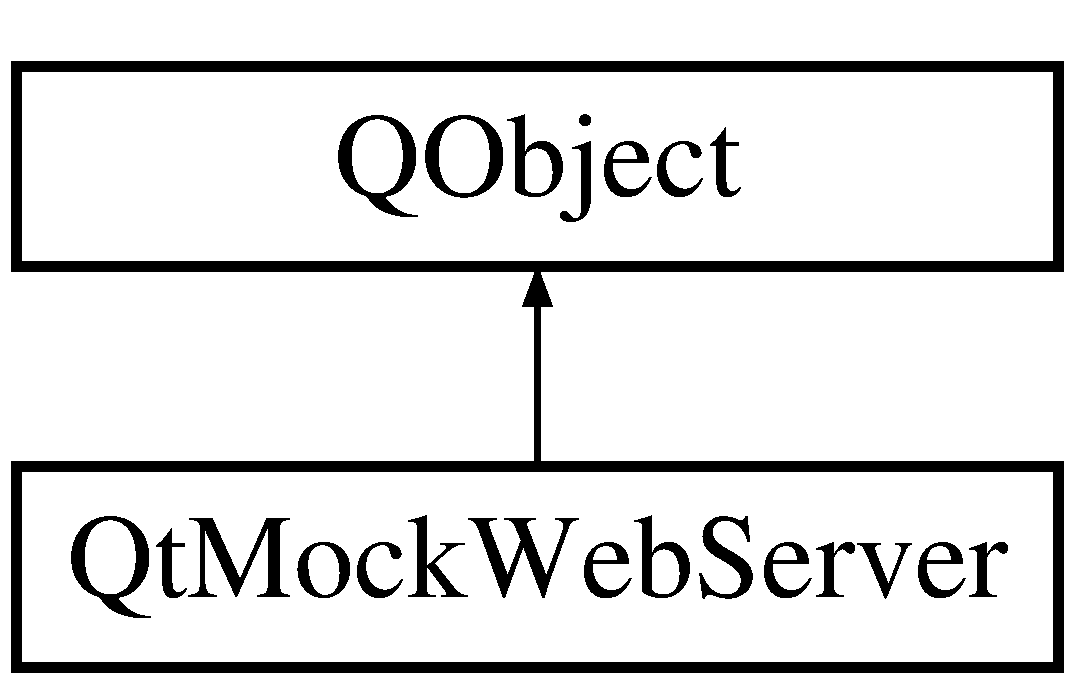
\includegraphics[height=2.000000cm]{class_qt_mock_web_server}
\end{center}
\end{figure}
\subsection*{Public Member Functions}
\begin{DoxyCompactItemize}
\item 
int \hyperlink{class_qt_mock_web_server_a83034aa1dbf8114d6b1bc01dd97cd2f3}{port} () const 
\begin{DoxyCompactList}\small\item\em Port of the mock server listening. Note that it's only avaliable after server started by \hyperlink{class_qt_mock_web_server_a5bad6c701969176fefd90d47417981c5}{play()}. \end{DoxyCompactList}\item 
Q\+String \hyperlink{class_qt_mock_web_server_a4779ef849c0bda6a605f453c8752491d}{host\+Name} () const 
\begin{DoxyCompactList}\small\item\em host name of the mock server listening. Note that it's only available after server started by \hyperlink{class_qt_mock_web_server_a5bad6c701969176fefd90d47417981c5}{play()}. \end{DoxyCompactList}\item 
Q\+Url \hyperlink{class_qt_mock_web_server_ace67dccbdce71316237a03e9830d8170}{get\+Url} (const Q\+String \&path)
\begin{DoxyCompactList}\small\item\em Get absolute url of given path. Note that it's only available after server started by \hyperlink{class_qt_mock_web_server_a5bad6c701969176fefd90d47417981c5}{play()}. \end{DoxyCompactList}\item 
void \hyperlink{class_qt_mock_web_server_a9b3f8f6054887c147b2c3fb36fbce271}{set\+Body\+Limit} (int max\+Body\+Length)
\begin{DoxyCompactList}\small\item\em Set max length limit of response body. \end{DoxyCompactList}\item 
\hyperlink{class_recorded_request}{Recorded\+Request} \hyperlink{class_qt_mock_web_server_aa1483ddd073de09247c53c0aa3a7b05b}{take\+Request} ()
\begin{DoxyCompactList}\small\item\em Take next recorded request the server received. \end{DoxyCompactList}\item 
int \hyperlink{class_qt_mock_web_server_a3d0745d34a224fcf31042d5b5438bbc6}{request\+Count} () const 
\begin{DoxyCompactList}\small\item\em Count of requests the server received. \end{DoxyCompactList}\item 
void \hyperlink{class_qt_mock_web_server_abb8bebe8b9db1d772ea84b244e64f138}{enqueue} (const \hyperlink{class_mock_response}{Mock\+Response} \&response)
\begin{DoxyCompactList}\small\item\em Enqueue a mock response to be served. \end{DoxyCompactList}\item 
\hypertarget{class_qt_mock_web_server_a5bad6c701969176fefd90d47417981c5}{void \hyperlink{class_qt_mock_web_server_a5bad6c701969176fefd90d47417981c5}{play} ()}\label{class_qt_mock_web_server_a5bad6c701969176fefd90d47417981c5}

\begin{DoxyCompactList}\small\item\em Start the server. \end{DoxyCompactList}\item 
void \hyperlink{class_qt_mock_web_server_a879a7db2d5b375323bdb464a6031084d}{play} (int \hyperlink{class_qt_mock_web_server_a83034aa1dbf8114d6b1bc01dd97cd2f3}{port})
\begin{DoxyCompactList}\small\item\em Try to start the server on given port. \end{DoxyCompactList}\item 
\hypertarget{class_qt_mock_web_server_a65f0a8d5b67723a4631fcf2741c787ff}{void \hyperlink{class_qt_mock_web_server_a65f0a8d5b67723a4631fcf2741c787ff}{shutdown} ()}\label{class_qt_mock_web_server_a65f0a8d5b67723a4631fcf2741c787ff}

\begin{DoxyCompactList}\small\item\em Shut down the server. \end{DoxyCompactList}\item 
void \hyperlink{class_qt_mock_web_server_af035f3eee01d9b857923d917f6b57098}{set\+Dispatcher} (\hyperlink{class_dispatcher}{Dispatcher} $\ast$dispatcher)
\begin{DoxyCompactList}\small\item\em Set a custom dispatcher which decides how to serve requests. \end{DoxyCompactList}\end{DoxyCompactItemize}


\subsection{Detailed Description}
A mock web server serving requests using pre-\/queued mock responses by default. 

\subsection{Member Function Documentation}
\hypertarget{class_qt_mock_web_server_abb8bebe8b9db1d772ea84b244e64f138}{\index{Qt\+Mock\+Web\+Server@{Qt\+Mock\+Web\+Server}!enqueue@{enqueue}}
\index{enqueue@{enqueue}!Qt\+Mock\+Web\+Server@{Qt\+Mock\+Web\+Server}}
\subsubsection[{enqueue}]{\setlength{\rightskip}{0pt plus 5cm}void Qt\+Mock\+Web\+Server\+::enqueue (
\begin{DoxyParamCaption}
\item[{const {\bf Mock\+Response} \&}]{response}
\end{DoxyParamCaption}
)}}\label{class_qt_mock_web_server_abb8bebe8b9db1d772ea84b244e64f138}


Enqueue a mock response to be served. 


\begin{DoxyParams}{Parameters}
{\em response} & The mock response. \\
\hline
\end{DoxyParams}
\hypertarget{class_qt_mock_web_server_ace67dccbdce71316237a03e9830d8170}{\index{Qt\+Mock\+Web\+Server@{Qt\+Mock\+Web\+Server}!get\+Url@{get\+Url}}
\index{get\+Url@{get\+Url}!Qt\+Mock\+Web\+Server@{Qt\+Mock\+Web\+Server}}
\subsubsection[{get\+Url}]{\setlength{\rightskip}{0pt plus 5cm}Q\+Url Qt\+Mock\+Web\+Server\+::get\+Url (
\begin{DoxyParamCaption}
\item[{const Q\+String \&}]{path}
\end{DoxyParamCaption}
)}}\label{class_qt_mock_web_server_ace67dccbdce71316237a03e9830d8170}


Get absolute url of given path. Note that it's only available after server started by \hyperlink{class_qt_mock_web_server_a5bad6c701969176fefd90d47417981c5}{play()}. 


\begin{DoxyParams}{Parameters}
{\em path} & Requested path. \\
\hline
\end{DoxyParams}
\begin{DoxyReturn}{Returns}
Absolute url of given path. 
\end{DoxyReturn}
\hypertarget{class_qt_mock_web_server_a4779ef849c0bda6a605f453c8752491d}{\index{Qt\+Mock\+Web\+Server@{Qt\+Mock\+Web\+Server}!host\+Name@{host\+Name}}
\index{host\+Name@{host\+Name}!Qt\+Mock\+Web\+Server@{Qt\+Mock\+Web\+Server}}
\subsubsection[{host\+Name}]{\setlength{\rightskip}{0pt plus 5cm}Q\+String Qt\+Mock\+Web\+Server\+::host\+Name (
\begin{DoxyParamCaption}
{}
\end{DoxyParamCaption}
) const}}\label{class_qt_mock_web_server_a4779ef849c0bda6a605f453c8752491d}


host name of the mock server listening. Note that it's only available after server started by \hyperlink{class_qt_mock_web_server_a5bad6c701969176fefd90d47417981c5}{play()}. 

\begin{DoxyReturn}{Returns}
Server host name. 
\end{DoxyReturn}
\hypertarget{class_qt_mock_web_server_a879a7db2d5b375323bdb464a6031084d}{\index{Qt\+Mock\+Web\+Server@{Qt\+Mock\+Web\+Server}!play@{play}}
\index{play@{play}!Qt\+Mock\+Web\+Server@{Qt\+Mock\+Web\+Server}}
\subsubsection[{play}]{\setlength{\rightskip}{0pt plus 5cm}void Qt\+Mock\+Web\+Server\+::play (
\begin{DoxyParamCaption}
\item[{int}]{port}
\end{DoxyParamCaption}
)}}\label{class_qt_mock_web_server_a879a7db2d5b375323bdb464a6031084d}


Try to start the server on given port. 


\begin{DoxyParams}{Parameters}
{\em port} & Start the server on this port. \\
\hline
\end{DoxyParams}
\hypertarget{class_qt_mock_web_server_a83034aa1dbf8114d6b1bc01dd97cd2f3}{\index{Qt\+Mock\+Web\+Server@{Qt\+Mock\+Web\+Server}!port@{port}}
\index{port@{port}!Qt\+Mock\+Web\+Server@{Qt\+Mock\+Web\+Server}}
\subsubsection[{port}]{\setlength{\rightskip}{0pt plus 5cm}int Qt\+Mock\+Web\+Server\+::port (
\begin{DoxyParamCaption}
{}
\end{DoxyParamCaption}
) const}}\label{class_qt_mock_web_server_a83034aa1dbf8114d6b1bc01dd97cd2f3}


Port of the mock server listening. Note that it's only avaliable after server started by \hyperlink{class_qt_mock_web_server_a5bad6c701969176fefd90d47417981c5}{play()}. 

\begin{DoxyReturn}{Returns}
Server port number 
\end{DoxyReturn}
\hypertarget{class_qt_mock_web_server_a3d0745d34a224fcf31042d5b5438bbc6}{\index{Qt\+Mock\+Web\+Server@{Qt\+Mock\+Web\+Server}!request\+Count@{request\+Count}}
\index{request\+Count@{request\+Count}!Qt\+Mock\+Web\+Server@{Qt\+Mock\+Web\+Server}}
\subsubsection[{request\+Count}]{\setlength{\rightskip}{0pt plus 5cm}int Qt\+Mock\+Web\+Server\+::request\+Count (
\begin{DoxyParamCaption}
{}
\end{DoxyParamCaption}
) const}}\label{class_qt_mock_web_server_a3d0745d34a224fcf31042d5b5438bbc6}


Count of requests the server received. 

\begin{DoxyReturn}{Returns}
Count of requests. 
\end{DoxyReturn}
\hypertarget{class_qt_mock_web_server_a9b3f8f6054887c147b2c3fb36fbce271}{\index{Qt\+Mock\+Web\+Server@{Qt\+Mock\+Web\+Server}!set\+Body\+Limit@{set\+Body\+Limit}}
\index{set\+Body\+Limit@{set\+Body\+Limit}!Qt\+Mock\+Web\+Server@{Qt\+Mock\+Web\+Server}}
\subsubsection[{set\+Body\+Limit}]{\setlength{\rightskip}{0pt plus 5cm}void Qt\+Mock\+Web\+Server\+::set\+Body\+Limit (
\begin{DoxyParamCaption}
\item[{int}]{max\+Body\+Length}
\end{DoxyParamCaption}
)}}\label{class_qt_mock_web_server_a9b3f8f6054887c147b2c3fb36fbce271}


Set max length limit of response body. 

\begin{DoxyRefDesc}{Todo}
\item[\hyperlink{todo__todo000001}{Todo}]Not fully implemented. \end{DoxyRefDesc}

\begin{DoxyParams}{Parameters}
{\em max\+Body\+Length} & Max body length limit. \\
\hline
\end{DoxyParams}
\hypertarget{class_qt_mock_web_server_af035f3eee01d9b857923d917f6b57098}{\index{Qt\+Mock\+Web\+Server@{Qt\+Mock\+Web\+Server}!set\+Dispatcher@{set\+Dispatcher}}
\index{set\+Dispatcher@{set\+Dispatcher}!Qt\+Mock\+Web\+Server@{Qt\+Mock\+Web\+Server}}
\subsubsection[{set\+Dispatcher}]{\setlength{\rightskip}{0pt plus 5cm}void Qt\+Mock\+Web\+Server\+::set\+Dispatcher (
\begin{DoxyParamCaption}
\item[{{\bf Dispatcher} $\ast$}]{dispatcher}
\end{DoxyParamCaption}
)}}\label{class_qt_mock_web_server_af035f3eee01d9b857923d917f6b57098}


Set a custom dispatcher which decides how to serve requests. 


\begin{DoxyParams}{Parameters}
{\em dispatcher} & The custome dispatcher. \\
\hline
\end{DoxyParams}
\hypertarget{class_qt_mock_web_server_aa1483ddd073de09247c53c0aa3a7b05b}{\index{Qt\+Mock\+Web\+Server@{Qt\+Mock\+Web\+Server}!take\+Request@{take\+Request}}
\index{take\+Request@{take\+Request}!Qt\+Mock\+Web\+Server@{Qt\+Mock\+Web\+Server}}
\subsubsection[{take\+Request}]{\setlength{\rightskip}{0pt plus 5cm}{\bf Recorded\+Request} Qt\+Mock\+Web\+Server\+::take\+Request (
\begin{DoxyParamCaption}
{}
\end{DoxyParamCaption}
)}}\label{class_qt_mock_web_server_aa1483ddd073de09247c53c0aa3a7b05b}


Take next recorded request the server received. 

\begin{DoxyReturn}{Returns}
Next recorded request. 
\end{DoxyReturn}


The documentation for this class was generated from the following files\+:\begin{DoxyCompactItemize}
\item 
src/Qt\+Mock\+Web\+Server.\+h\item 
src/Qt\+Mock\+Web\+Server.\+cpp\end{DoxyCompactItemize}

\hypertarget{class_queue_dispatcher}{\section{Queue\+Dispatcher Class Reference}
\label{class_queue_dispatcher}\index{Queue\+Dispatcher@{Queue\+Dispatcher}}
}


A dispatcher using queue policy.  




{\ttfamily \#include $<$Queue\+Dispatcher.\+h$>$}

Inheritance diagram for Queue\+Dispatcher\+:\begin{figure}[H]
\begin{center}
\leavevmode
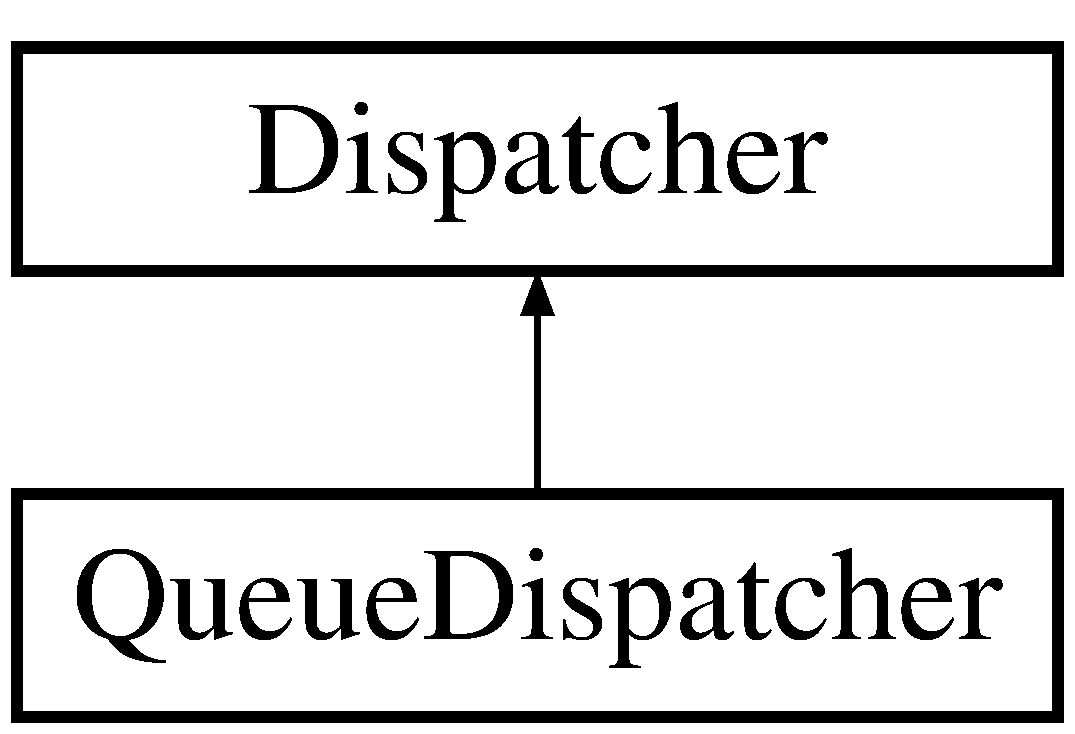
\includegraphics[height=2.000000cm]{class_queue_dispatcher}
\end{center}
\end{figure}
\subsection*{Public Member Functions}
\begin{DoxyCompactItemize}
\item 
virtual \hyperlink{class_mock_response}{Mock\+Response} \hyperlink{class_queue_dispatcher_ae5fe9ec67b24b75ece3f28d908e2764e}{dispatch} (const \hyperlink{class_recorded_request}{Recorded\+Request} \&request)
\begin{DoxyCompactList}\small\item\em Serve incoming request with next response in queue. \end{DoxyCompactList}\item 
virtual \hyperlink{class_mock_response}{Mock\+Response} \hyperlink{class_queue_dispatcher_acea23f016b5fd62ec7cc94ee1db1816e}{peek} ()
\begin{DoxyCompactList}\small\item\em Head response in queue if queue is not empty. Otherwise the fail-\/fast response is returned if set. If both are empty, \hyperlink{class_dispatcher_af4768d8abe65389a5cdbb48499c32a0f}{Dispatcher\+::peek()} is returned. \end{DoxyCompactList}\item 
void \hyperlink{class_queue_dispatcher_a5ce0e46fe53d760fe98da7ec010dc0ef}{enqueue\+Response} (const \hyperlink{class_mock_response}{Mock\+Response} \&response)
\begin{DoxyCompactList}\small\item\em Enqueue given response. \end{DoxyCompactList}\item 
void \hyperlink{class_queue_dispatcher_a2f09193b180fb46fe7b0822022b52222}{set\+Fail\+Fast} (bool fail\+Fast)
\begin{DoxyCompactList}\small\item\em Set if we should dispatch a immediate fail response when the queue is empty. \end{DoxyCompactList}\item 
void \hyperlink{class_queue_dispatcher_ab7a07e38d21032f2657896c647cb6f2f}{set\+Fail\+Fast} (\hyperlink{class_mock_response}{Mock\+Response} $\ast$fail\+Fast\+Response)
\begin{DoxyCompactList}\small\item\em Set the fail-\/fast response which will be used when the queue is empty. \end{DoxyCompactList}\end{DoxyCompactItemize}
\subsection*{Protected Attributes}
\begin{DoxyCompactItemize}
\item 
\hypertarget{class_queue_dispatcher_aa844b856cedb4439abaf022118a7dc50}{Q\+Queue$<$ \hyperlink{class_mock_response}{Mock\+Response} $>$ {\bfseries m\+\_\+response\+Queue}}\label{class_queue_dispatcher_aa844b856cedb4439abaf022118a7dc50}

\end{DoxyCompactItemize}


\subsection{Detailed Description}
A dispatcher using queue policy. 

\subsection{Member Function Documentation}
\hypertarget{class_queue_dispatcher_ae5fe9ec67b24b75ece3f28d908e2764e}{\index{Queue\+Dispatcher@{Queue\+Dispatcher}!dispatch@{dispatch}}
\index{dispatch@{dispatch}!Queue\+Dispatcher@{Queue\+Dispatcher}}
\subsubsection[{dispatch}]{\setlength{\rightskip}{0pt plus 5cm}{\bf Mock\+Response} Queue\+Dispatcher\+::dispatch (
\begin{DoxyParamCaption}
\item[{const {\bf Recorded\+Request} \&}]{request}
\end{DoxyParamCaption}
)\hspace{0.3cm}{\ttfamily [virtual]}}}\label{class_queue_dispatcher_ae5fe9ec67b24b75ece3f28d908e2764e}


Serve incoming request with next response in queue. 


\begin{DoxyParams}{Parameters}
{\em request} & The incoming request. \\
\hline
\end{DoxyParams}
\begin{DoxyReturn}{Returns}
Next response in queue. 
\end{DoxyReturn}


Implements \hyperlink{class_dispatcher_acbbf8d0ca649be337d805dcbaf4ba81b}{Dispatcher}.

\hypertarget{class_queue_dispatcher_a5ce0e46fe53d760fe98da7ec010dc0ef}{\index{Queue\+Dispatcher@{Queue\+Dispatcher}!enqueue\+Response@{enqueue\+Response}}
\index{enqueue\+Response@{enqueue\+Response}!Queue\+Dispatcher@{Queue\+Dispatcher}}
\subsubsection[{enqueue\+Response}]{\setlength{\rightskip}{0pt plus 5cm}void Queue\+Dispatcher\+::enqueue\+Response (
\begin{DoxyParamCaption}
\item[{const {\bf Mock\+Response} \&}]{response}
\end{DoxyParamCaption}
)}}\label{class_queue_dispatcher_a5ce0e46fe53d760fe98da7ec010dc0ef}


Enqueue given response. 


\begin{DoxyParams}{Parameters}
{\em response} & A mock response. \\
\hline
\end{DoxyParams}
\hypertarget{class_queue_dispatcher_acea23f016b5fd62ec7cc94ee1db1816e}{\index{Queue\+Dispatcher@{Queue\+Dispatcher}!peek@{peek}}
\index{peek@{peek}!Queue\+Dispatcher@{Queue\+Dispatcher}}
\subsubsection[{peek}]{\setlength{\rightskip}{0pt plus 5cm}{\bf Mock\+Response} Queue\+Dispatcher\+::peek (
\begin{DoxyParamCaption}
{}
\end{DoxyParamCaption}
)\hspace{0.3cm}{\ttfamily [virtual]}}}\label{class_queue_dispatcher_acea23f016b5fd62ec7cc94ee1db1816e}


Head response in queue if queue is not empty. Otherwise the fail-\/fast response is returned if set. If both are empty, \hyperlink{class_dispatcher_af4768d8abe65389a5cdbb48499c32a0f}{Dispatcher\+::peek()} is returned. 

\begin{DoxyReturn}{Returns}
Guess of next resposne. 
\end{DoxyReturn}


Reimplemented from \hyperlink{class_dispatcher_af4768d8abe65389a5cdbb48499c32a0f}{Dispatcher}.

\hypertarget{class_queue_dispatcher_a2f09193b180fb46fe7b0822022b52222}{\index{Queue\+Dispatcher@{Queue\+Dispatcher}!set\+Fail\+Fast@{set\+Fail\+Fast}}
\index{set\+Fail\+Fast@{set\+Fail\+Fast}!Queue\+Dispatcher@{Queue\+Dispatcher}}
\subsubsection[{set\+Fail\+Fast}]{\setlength{\rightskip}{0pt plus 5cm}void Queue\+Dispatcher\+::set\+Fail\+Fast (
\begin{DoxyParamCaption}
\item[{bool}]{fail\+Fast}
\end{DoxyParamCaption}
)}}\label{class_queue_dispatcher_a2f09193b180fb46fe7b0822022b52222}


Set if we should dispatch a immediate fail response when the queue is empty. 

\begin{DoxyRefDesc}{Todo}
\item[\hyperlink{todo__todo000002}{Todo}]It will be useful after queue is implemented blockable. \end{DoxyRefDesc}

\begin{DoxyParams}{Parameters}
{\em fail\+Fast} & True if should fail fast. \\
\hline
\end{DoxyParams}
\hypertarget{class_queue_dispatcher_ab7a07e38d21032f2657896c647cb6f2f}{\index{Queue\+Dispatcher@{Queue\+Dispatcher}!set\+Fail\+Fast@{set\+Fail\+Fast}}
\index{set\+Fail\+Fast@{set\+Fail\+Fast}!Queue\+Dispatcher@{Queue\+Dispatcher}}
\subsubsection[{set\+Fail\+Fast}]{\setlength{\rightskip}{0pt plus 5cm}void Queue\+Dispatcher\+::set\+Fail\+Fast (
\begin{DoxyParamCaption}
\item[{{\bf Mock\+Response} $\ast$}]{fail\+Fast\+Response}
\end{DoxyParamCaption}
)}}\label{class_queue_dispatcher_ab7a07e38d21032f2657896c647cb6f2f}


Set the fail-\/fast response which will be used when the queue is empty. 

\begin{DoxyRefDesc}{Todo}
\item[\hyperlink{todo__todo000003}{Todo}]It will be useful after queue is implemented blockable. \end{DoxyRefDesc}

\begin{DoxyParams}{Parameters}
{\em fail\+Fast\+Response} & \\
\hline
\end{DoxyParams}


The documentation for this class was generated from the following files\+:\begin{DoxyCompactItemize}
\item 
src/Queue\+Dispatcher.\+h\item 
src/Queue\+Dispatcher.\+cpp\end{DoxyCompactItemize}

\hypertarget{class_recorded_request}{\section{Recorded\+Request Class Reference}
\label{class_recorded_request}\index{Recorded\+Request@{Recorded\+Request}}
}


The recorded request to be validated.  




{\ttfamily \#include $<$Recorded\+Request.\+h$>$}

\subsection*{Public Member Functions}
\begin{DoxyCompactItemize}
\item 
\hypertarget{class_recorded_request_aca317e0e665c6455c3307ae09d67fbdb}{{\bfseries Recorded\+Request} (const Q\+String \&\hyperlink{class_recorded_request_ab2324bf506aa3e1004d161ea5e5ab97e}{request\+Line}, const Q\+List$<$ Q\+String $>$ \&\hyperlink{class_recorded_request_a3ed5bf33c7903c9078e49eae577d127b}{headers}, const Q\+List$<$ int $>$ \&\hyperlink{class_recorded_request_a5335457575099741e9cc75dc0f266a3d}{chunk\+Sizes}, long \hyperlink{class_recorded_request_ae3092b418550fc6d83fb7add89e54a34}{body\+Size}, const Q\+Byte\+Array \&\hyperlink{class_recorded_request_a29a9250993cbf1c33ad427f08ca936cf}{body}, int \hyperlink{class_recorded_request_af40b9720c9aa0074555dbccc43a37d2a}{sequence\+Number})}\label{class_recorded_request_aca317e0e665c6455c3307ae09d67fbdb}

\item 
bool \hyperlink{class_recorded_request_ae79ac696d5a57db8102789eb1f0929f4}{is\+Null} () const 
\begin{DoxyCompactList}\small\item\em Check if empty. \end{DoxyCompactList}\item 
Q\+String \hyperlink{class_recorded_request_ab2324bf506aa3e1004d161ea5e5ab97e}{request\+Line} () const 
\begin{DoxyCompactList}\small\item\em The request line. \end{DoxyCompactList}\item 
Q\+String \hyperlink{class_recorded_request_a3d84b8e2b214b74d4c6e1f8e3df098c2}{method} () const 
\begin{DoxyCompactList}\small\item\em The request method such as \char`\"{}\+G\+E\+T\char`\"{}/\char`\"{}\+P\+O\+S\+T\char`\"{}, etc. \end{DoxyCompactList}\item 
Q\+String \hyperlink{class_recorded_request_a77f871f46f16551e2d49e2d8500f8a21}{path} () const 
\begin{DoxyCompactList}\small\item\em The request path such as \char`\"{}/index.\+html\char`\"{}. \end{DoxyCompactList}\item 
Q\+List$<$ Q\+String $>$ \hyperlink{class_recorded_request_a3ed5bf33c7903c9078e49eae577d127b}{headers} () const 
\begin{DoxyCompactList}\small\item\em A list of request headers. \end{DoxyCompactList}\item 
Q\+String \hyperlink{class_recorded_request_ac609ec48565b1b46752d777d06ea6134}{header} (const Q\+String \&name) const 
\begin{DoxyCompactList}\small\item\em Value of given header name. \end{DoxyCompactList}\item 
Q\+List$<$ Q\+String $>$ \hyperlink{class_recorded_request_a851d5972e3e330ff75b84d514eccb51e}{headers} (const Q\+String \&name) const 
\begin{DoxyCompactList}\small\item\em A list of values of given header name. Headers such as \char`\"{}\+Cookies\char`\"{} may have multiple ones. \end{DoxyCompactList}\item 
Q\+List$<$ int $>$ \hyperlink{class_recorded_request_a5335457575099741e9cc75dc0f266a3d}{chunk\+Sizes} () const 
\begin{DoxyCompactList}\small\item\em Sizes of each body chunk. \end{DoxyCompactList}\item 
long \hyperlink{class_recorded_request_ae3092b418550fc6d83fb7add89e54a34}{body\+Size} () const 
\begin{DoxyCompactList}\small\item\em Size of request body. \end{DoxyCompactList}\item 
Q\+Byte\+Array \hyperlink{class_recorded_request_a29a9250993cbf1c33ad427f08ca936cf}{body} () const 
\begin{DoxyCompactList}\small\item\em Content of request body. \end{DoxyCompactList}\item 
Q\+String \hyperlink{class_recorded_request_a745e3caa89e0e44f962b47d67c9fafdd}{utf8\+Body} () const 
\begin{DoxyCompactList}\small\item\em String of request body decoded using \char`\"{}\+U\+T\+F-\/8\char`\"{}. \end{DoxyCompactList}\item 
int \hyperlink{class_recorded_request_af40b9720c9aa0074555dbccc43a37d2a}{sequence\+Number} () const 
\begin{DoxyCompactList}\small\item\em Sequence number of this request. \end{DoxyCompactList}\end{DoxyCompactItemize}


\subsection{Detailed Description}
The recorded request to be validated. 

\subsection{Member Function Documentation}
\hypertarget{class_recorded_request_a29a9250993cbf1c33ad427f08ca936cf}{\index{Recorded\+Request@{Recorded\+Request}!body@{body}}
\index{body@{body}!Recorded\+Request@{Recorded\+Request}}
\subsubsection[{body}]{\setlength{\rightskip}{0pt plus 5cm}Q\+Byte\+Array Recorded\+Request\+::body (
\begin{DoxyParamCaption}
{}
\end{DoxyParamCaption}
) const}}\label{class_recorded_request_a29a9250993cbf1c33ad427f08ca936cf}


Content of request body. 

\begin{DoxyReturn}{Returns}
Content of request body. 
\end{DoxyReturn}
\hypertarget{class_recorded_request_ae3092b418550fc6d83fb7add89e54a34}{\index{Recorded\+Request@{Recorded\+Request}!body\+Size@{body\+Size}}
\index{body\+Size@{body\+Size}!Recorded\+Request@{Recorded\+Request}}
\subsubsection[{body\+Size}]{\setlength{\rightskip}{0pt plus 5cm}long Recorded\+Request\+::body\+Size (
\begin{DoxyParamCaption}
{}
\end{DoxyParamCaption}
) const}}\label{class_recorded_request_ae3092b418550fc6d83fb7add89e54a34}


Size of request body. 

\begin{DoxyReturn}{Returns}
Size of request body. 
\end{DoxyReturn}
\hypertarget{class_recorded_request_a5335457575099741e9cc75dc0f266a3d}{\index{Recorded\+Request@{Recorded\+Request}!chunk\+Sizes@{chunk\+Sizes}}
\index{chunk\+Sizes@{chunk\+Sizes}!Recorded\+Request@{Recorded\+Request}}
\subsubsection[{chunk\+Sizes}]{\setlength{\rightskip}{0pt plus 5cm}Q\+List$<$ int $>$ Recorded\+Request\+::chunk\+Sizes (
\begin{DoxyParamCaption}
{}
\end{DoxyParamCaption}
) const}}\label{class_recorded_request_a5335457575099741e9cc75dc0f266a3d}


Sizes of each body chunk. 

\begin{DoxyReturn}{Returns}
Sizes of each body chunk. 
\end{DoxyReturn}
\hypertarget{class_recorded_request_ac609ec48565b1b46752d777d06ea6134}{\index{Recorded\+Request@{Recorded\+Request}!header@{header}}
\index{header@{header}!Recorded\+Request@{Recorded\+Request}}
\subsubsection[{header}]{\setlength{\rightskip}{0pt plus 5cm}Q\+String Recorded\+Request\+::header (
\begin{DoxyParamCaption}
\item[{const Q\+String \&}]{name}
\end{DoxyParamCaption}
) const}}\label{class_recorded_request_ac609ec48565b1b46752d777d06ea6134}


Value of given header name. 


\begin{DoxyParams}{Parameters}
{\em name} & Header name. \\
\hline
\end{DoxyParams}
\begin{DoxyReturn}{Returns}
Value of given header name. 
\end{DoxyReturn}
\hypertarget{class_recorded_request_a3ed5bf33c7903c9078e49eae577d127b}{\index{Recorded\+Request@{Recorded\+Request}!headers@{headers}}
\index{headers@{headers}!Recorded\+Request@{Recorded\+Request}}
\subsubsection[{headers}]{\setlength{\rightskip}{0pt plus 5cm}Q\+List$<$ Q\+String $>$ Recorded\+Request\+::headers (
\begin{DoxyParamCaption}
{}
\end{DoxyParamCaption}
) const}}\label{class_recorded_request_a3ed5bf33c7903c9078e49eae577d127b}


A list of request headers. 

\begin{DoxyReturn}{Returns}
A list of request headers. 
\end{DoxyReturn}
\hypertarget{class_recorded_request_a851d5972e3e330ff75b84d514eccb51e}{\index{Recorded\+Request@{Recorded\+Request}!headers@{headers}}
\index{headers@{headers}!Recorded\+Request@{Recorded\+Request}}
\subsubsection[{headers}]{\setlength{\rightskip}{0pt plus 5cm}Q\+List$<$ Q\+String $>$ Recorded\+Request\+::headers (
\begin{DoxyParamCaption}
\item[{const Q\+String \&}]{name}
\end{DoxyParamCaption}
) const}}\label{class_recorded_request_a851d5972e3e330ff75b84d514eccb51e}


A list of values of given header name. Headers such as \char`\"{}\+Cookies\char`\"{} may have multiple ones. 


\begin{DoxyParams}{Parameters}
{\em name} & Header name. \\
\hline
\end{DoxyParams}
\begin{DoxyReturn}{Returns}
A list of values. 
\end{DoxyReturn}
\hypertarget{class_recorded_request_ae79ac696d5a57db8102789eb1f0929f4}{\index{Recorded\+Request@{Recorded\+Request}!is\+Null@{is\+Null}}
\index{is\+Null@{is\+Null}!Recorded\+Request@{Recorded\+Request}}
\subsubsection[{is\+Null}]{\setlength{\rightskip}{0pt plus 5cm}bool Recorded\+Request\+::is\+Null (
\begin{DoxyParamCaption}
{}
\end{DoxyParamCaption}
) const}}\label{class_recorded_request_ae79ac696d5a57db8102789eb1f0929f4}


Check if empty. 

\begin{DoxyReturn}{Returns}
True if empty. 
\end{DoxyReturn}
\hypertarget{class_recorded_request_a3d84b8e2b214b74d4c6e1f8e3df098c2}{\index{Recorded\+Request@{Recorded\+Request}!method@{method}}
\index{method@{method}!Recorded\+Request@{Recorded\+Request}}
\subsubsection[{method}]{\setlength{\rightskip}{0pt plus 5cm}Q\+String Recorded\+Request\+::method (
\begin{DoxyParamCaption}
{}
\end{DoxyParamCaption}
) const}}\label{class_recorded_request_a3d84b8e2b214b74d4c6e1f8e3df098c2}


The request method such as \char`\"{}\+G\+E\+T\char`\"{}/\char`\"{}\+P\+O\+S\+T\char`\"{}, etc. 

\begin{DoxyReturn}{Returns}
The request method. 
\end{DoxyReturn}
\hypertarget{class_recorded_request_a77f871f46f16551e2d49e2d8500f8a21}{\index{Recorded\+Request@{Recorded\+Request}!path@{path}}
\index{path@{path}!Recorded\+Request@{Recorded\+Request}}
\subsubsection[{path}]{\setlength{\rightskip}{0pt plus 5cm}Q\+String Recorded\+Request\+::path (
\begin{DoxyParamCaption}
{}
\end{DoxyParamCaption}
) const}}\label{class_recorded_request_a77f871f46f16551e2d49e2d8500f8a21}


The request path such as \char`\"{}/index.\+html\char`\"{}. 

\begin{DoxyReturn}{Returns}
The request path. 
\end{DoxyReturn}
\hypertarget{class_recorded_request_ab2324bf506aa3e1004d161ea5e5ab97e}{\index{Recorded\+Request@{Recorded\+Request}!request\+Line@{request\+Line}}
\index{request\+Line@{request\+Line}!Recorded\+Request@{Recorded\+Request}}
\subsubsection[{request\+Line}]{\setlength{\rightskip}{0pt plus 5cm}Q\+String Recorded\+Request\+::request\+Line (
\begin{DoxyParamCaption}
{}
\end{DoxyParamCaption}
) const}}\label{class_recorded_request_ab2324bf506aa3e1004d161ea5e5ab97e}


The request line. 

\begin{DoxyReturn}{Returns}
The request line. 
\end{DoxyReturn}
\hypertarget{class_recorded_request_af40b9720c9aa0074555dbccc43a37d2a}{\index{Recorded\+Request@{Recorded\+Request}!sequence\+Number@{sequence\+Number}}
\index{sequence\+Number@{sequence\+Number}!Recorded\+Request@{Recorded\+Request}}
\subsubsection[{sequence\+Number}]{\setlength{\rightskip}{0pt plus 5cm}int Recorded\+Request\+::sequence\+Number (
\begin{DoxyParamCaption}
{}
\end{DoxyParamCaption}
) const}}\label{class_recorded_request_af40b9720c9aa0074555dbccc43a37d2a}


Sequence number of this request. 

\begin{DoxyReturn}{Returns}
Sequence number of this request. 
\end{DoxyReturn}
\hypertarget{class_recorded_request_a745e3caa89e0e44f962b47d67c9fafdd}{\index{Recorded\+Request@{Recorded\+Request}!utf8\+Body@{utf8\+Body}}
\index{utf8\+Body@{utf8\+Body}!Recorded\+Request@{Recorded\+Request}}
\subsubsection[{utf8\+Body}]{\setlength{\rightskip}{0pt plus 5cm}Q\+String Recorded\+Request\+::utf8\+Body (
\begin{DoxyParamCaption}
{}
\end{DoxyParamCaption}
) const}}\label{class_recorded_request_a745e3caa89e0e44f962b47d67c9fafdd}


String of request body decoded using \char`\"{}\+U\+T\+F-\/8\char`\"{}. 

\begin{DoxyReturn}{Returns}
String of request body decoded using \char`\"{}\+U\+T\+F-\/8\char`\"{}. 
\end{DoxyReturn}


The documentation for this class was generated from the following files\+:\begin{DoxyCompactItemize}
\item 
src/Recorded\+Request.\+h\item 
src/Recorded\+Request.\+cpp\end{DoxyCompactItemize}

%--- End generated contents ---

% Index
\newpage
\phantomsection
\addcontentsline{toc}{chapter}{Index}
\printindex

\end{document}
